\documentclass[11pt]{article}
\usepackage{geometry}                % See geometry.pdf to learn the layout options. There are lots.
\geometry{letterpaper}                   % ... or a4paper or a5paper or ... 
%\geometry{landscape}                % Activate for for rotated page geometry
\usepackage[parfill]{parskip}    % Activate to begin paragraphs with an empty line rather than an indent
\usepackage{daves,fancyhdr,natbib,graphicx,dcolumn,amsmath,lastpage,url}
\usepackage{amsmath,amssymb,epstopdf,longtable}
\usepackage{paralist}  % need to properly formulate standard answer blocks
\usepackage[final]{pdfpages}
\DeclareGraphicsRule{.tif}{png}{.png}{`convert #1 `dirname #1`/`basename #1 .tif`.png}
\pagestyle{fancy}
\lhead{CE 3372 Water Systems Design; Exam 1}
\rhead{Name:\_\_\_\_\_\_\_\_\_\_\_\_\_\_\_\_\_\_\_\_\_\_\_\_\_\_\_\_\_\_\_\_\_\_}
\lfoot{SPRING 2017 A.}
\cfoot{}
\rfoot{Page \thepage\ of \pageref{LastPage}}
\renewcommand\headrulewidth{0pt}
\newcommand\tab[1][1cm]{\hspace*{#1}}



\begin{document}
%%%%%%%%%%%%%%%%%%%%%%%%%%%%%%%%%%%
%\begingroup
%\begin{center}
%{\textbf{{ CE 3372 Water Systems Design Exam 1 }} }
%\end{center}
%\endgroup

%%%%%%%%%%%%%%%%%%%%%%%%%%%

\begin{enumerate}
\item One acre is a square with sides of length of 208.71 feet.  How many square feet in an acre?
~\\
~\\
\item 1 inch is $~\approx 25.4$ millimeters.  What is the diameter of a six-inch pipe, in millimeters?
~\\
~\\
\item 1 meter is $~\approx 3.28$ feet.   There are 5280 feet in a mile.   How many meters in one mile?
~\\
~\\
~\\
~\\
\item One hectare is a square with sides of length 100 meters.  How many acres in one hectare?
~\\
~\\
~\\
~\\
~\\
\begin{figure}[h!] %  figure placement: here, top, bottom, or page
   \centering
   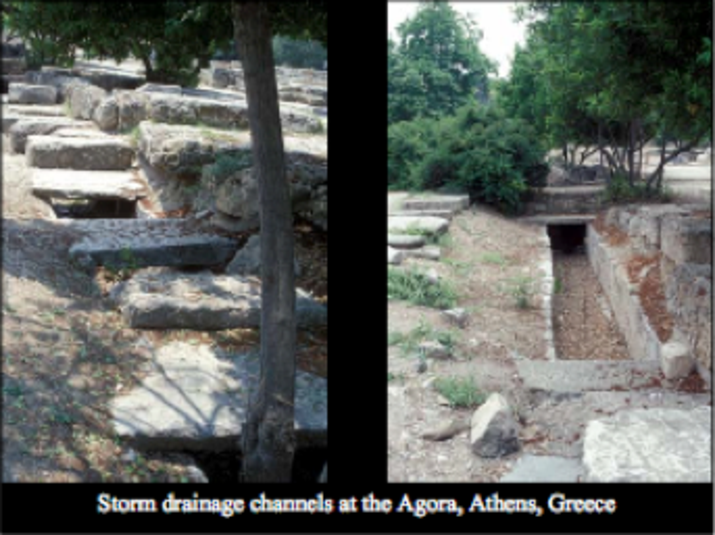
\includegraphics[height=2.5in]{greek-storm-drain.pdf} 
   \caption{Photograph of ancient storm drain}
   \label{fig:greek-storm-drain}
\end{figure}
\item Figure \ref{fig:greek-storm-drain} is a photograph of a
\begin{enumerate}[(a)]
\item Water use system
\item Water control system
\item Environmental restoration system
\item W{\"a}sserb{\"e}rger system
\end{enumerate}

\clearpage
\item Figure \ref{fig:SewerDrawing} is a portion of an engineering drawing of a gravity-flow wastewater conduit. 
\begin{figure}[h!] %  figure placement: here, top, bottom, or page
   \centering
   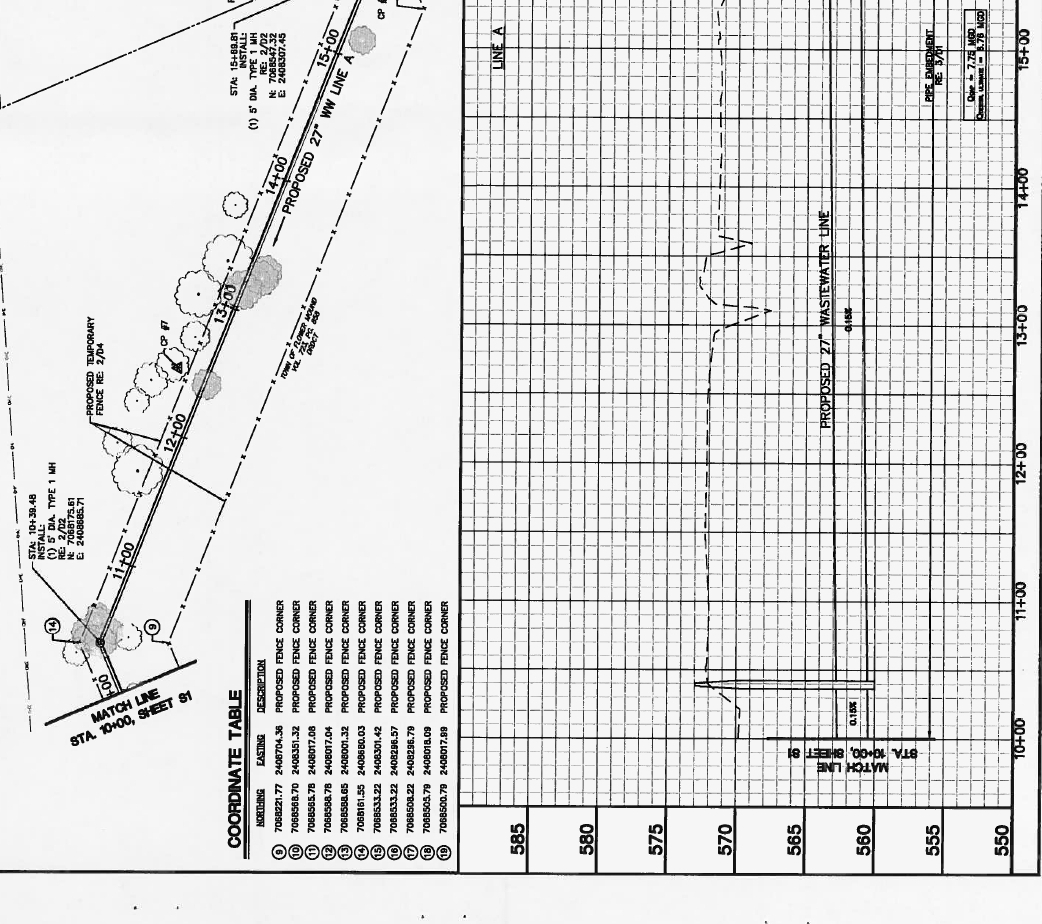
\includegraphics[height=6.2in]{SewerDrawing.jpg} 
   \caption{Engineering drawing of sanitary sewer system (display is rotated)}
   \label{fig:SewerDrawing}
\end{figure}

\begin{enumerate}[(a)]
\item What object is located at station 10+38.48?
\item What is the invert elevation of the pipe at station 13+00?
\item What is the diameter of the pipe in inches?
\item What direction is sewage intended to flow?
\end{enumerate}
\clearpage
%%%%%%%%%%%%%%%%%%%%
% Hazen-Williams Application (HIPS) %
%%%%%%%%%%%%%%%%%%%%
\item Equation \ref{eqn:hazen-williams} is the  Hazen-Williams discharge model for U.S. Customary units.
\begin{equation}
Q = 1.318~A~C_h~R^{0.63}~S^{0.54}
\label{eqn:hazen-williams}
\end{equation}

where;\\~\\
\tab $Q$ is the discharge in $ft^3/sec$;\\
\tab $A$ is the cross section area of pipe in $ft^2$ ($A = \frac{\pi D^2}{4}$; $D$ is the pipe diameter.);\\
\tab $C_h$ is the Hazen-Williams friction coefficient (depends on pipe roughness);\\
\tab $R$ is the hydraulic radius in $ft$; and \\
\tab $S$ is the slope of the energy grade line ($\frac{h_f}{L}$); $L$ is the length of pipe.

\begin{enumerate}[(a)]
\item Rearrange the equation in terms of head loss ($h_f = \dots$). ~\newpage
\item Estimate the head loss in a 12,000 foot length of 6-foot diameter, enamel coated steel pipe that carries carries 60$^o$F water at a discharge of 295 cubic-feet per second (cfs), using the Hazen-Williams head loss model.  Use a Hazen-Williams loss coefficient of $C_h~=150$.
\end{enumerate}
\clearpage
%%%%%%%%%%%%%%%%%%%
%   Jain Application (HIPS, MSMD)  %
%%%%%%%%%%%%%%%%%%%
\item 
Equation \ref{eqn:flow-jain} is an explicit formula (based on the Darcy-Weisbach head loss model and the Colebrook-White frictional loss equation)for estimating discharge from head loss and material properties. %\citep{jain1976}.
\begin{equation}
Q=-2.22D^{5/2} \times \sqrt{gh_f/L}\times[log_{10} (\frac{k_s}{3.7D} + \frac{1.78\nu}{D^{3/2}\sqrt{gh_f/L}} )]
\label{eqn:flow-jain}
\end{equation}

where;\\~\\
\tab $Q$ is the discharge in $L^3/T$;\\
\tab $D$ is the pipe diameter; \\
\tab $h_f$ is the head loss in the pipe; \\
\tab $g$ is the gravitational acceleration constant; \\
\tab $L$ is the length of pipe; \\
\tab $k_s$ is the pipe roughness height; \\
\tab $\nu$ is the kinematic viscosity of liquid in the pipe; \\ 



Water at 50$^o$F has kinematic viscosity of $1.45\times10^{-5}~ft^2/s$.   The sand roughness of ductile iron is $8.5\times10^{-4}~ft$.  

Determine:
\begin{enumerate}[(a)]
\item Depth of a column of water if the pressure at the bottom of the column is 21 psi? \newpage
\item Estimate the discharge in the 3.2 mile long, 24-inch diameter, ductile iron pipeline connecting points A and B depicted in Figure \ref{fig:PipePressureProblem}.  
Point A is 28 feet higher in elevation than point B.  The pressure at point B is 21 pounds per square-inch (psi) greater than the pressure at point A.

\begin{figure}[h!] %  figure placement: here, top, bottom, or page
   \centering
   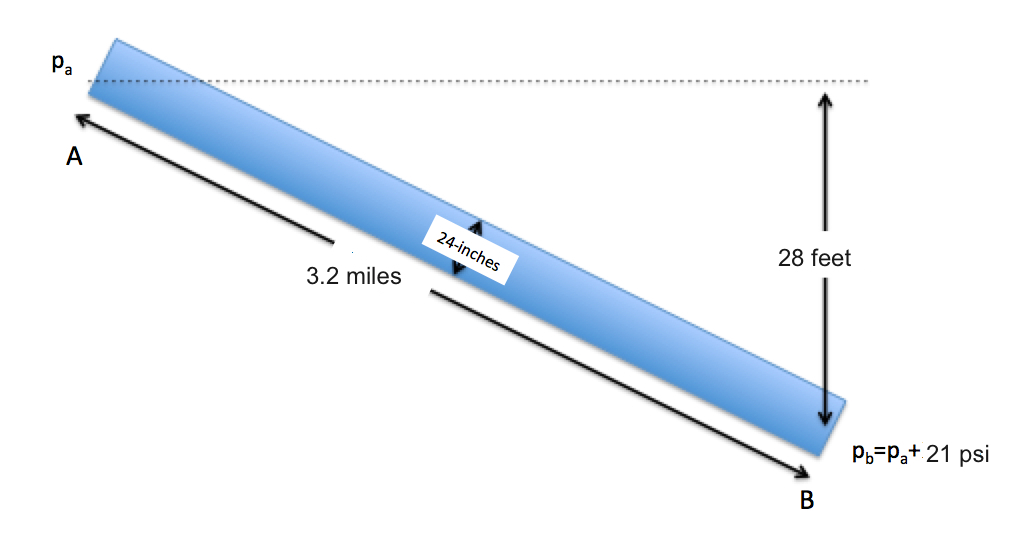
\includegraphics[width=4in]{PipePressureProblem.jpg} 
   \caption{Pipeline Schematic}
   \label{fig:PipePressureProblem}
\end{figure}

\end{enumerate}

\clearpage
%%%%%%%%%%%%%%%%%%
% Tehachapi Pipelines YOYO %%%
%%%%%%%%%%%%%%%%%%
\item Figure \ref{fig:parallelpipes} is an aerial image of a parallel pipeline system in California.   

\begin{figure}[htbp] %  figure placement: here, top, bottom, or page
   \centering
   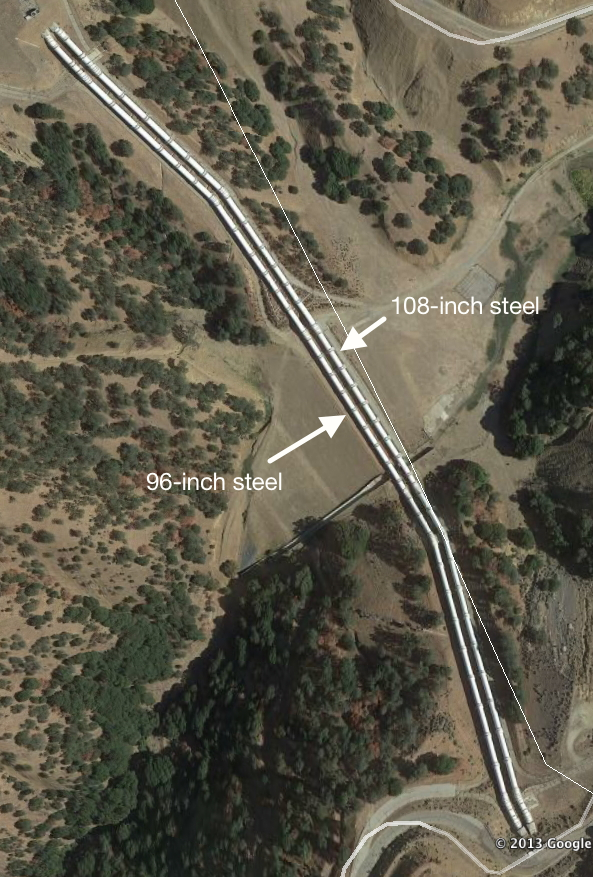
\includegraphics[width=2in]{parallelpipes.jpg} 
   \caption{Parallel Pipeline System}
   \label{fig:parallelpipes}
\end{figure}

The left pipeline is a 96-inch diameter steel pipe, whereas the right pipeline is a 108-inch diameter steel pipe.  
Water at 50$^o$F has kinematic viscosity of $1.45\times10^{-5}~ft^2/s$.   
The sand roughness of ductile iron is $1.64\times10^{-4}~ft$.   
If the head difference for the one-mile long pipelines between the thrust blocks is 100 feet, determine the discharge in each pipe in cubic-feet-per-second.
\clearpage
Problem 3 (continued)
\clearpage

%%%%%%%%%%%%%%%%%%%%%%%%%%%%%
%%%%%%%%%%%%%%%%%%%%%%%%%%%%%%%%%%%%%%%%%%%%%%%%%%
Figure \ref{fig:wheatstone_bridge} is a pipe network with the following properties:
\begin{figure}[h!] %  figure placement: here, top, bottom, or page
\centering
   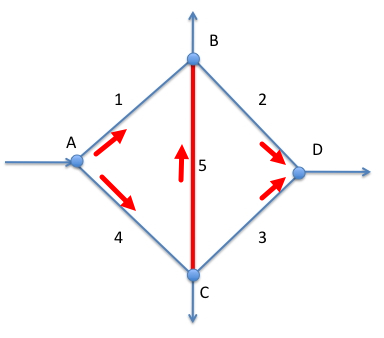
\includegraphics[width=5.5in]{wheatstone_bridge.jpg}
   \caption{Pipe network}
   \label{fig:wheatstone_bridge} 
\end{figure}

\begin{table}[h!]
\footnotesize
   \centering
   \caption{Network properties for Figure \ref{fig:wheatstone_bridge}}
\begin{tabular}{lll}
\hline
Node&Demand (cfs)&  Elevation(ft) \\
\hline
A & -0.60 & 0.00 \\
B &  0.15   & 0.00 \\
C & 0.15 & 0.00 \\
D & 0.30 & 0.00 \\
\hline
Pipe& Length (ft)&  Diameter (ft)\\
\hline
1 & 1000 & 3/12 \\
2 & 1000 & 3/12\\
3 & 1000 & 3/12\\
4 & 1000 & 3/12\\
5 & 1400 & 3/12\\
\end{tabular}
\label{tab:wheatstone1}
\normalsize
\end{table}
\clearpage

\item Referring to Figure \ref{fig:wheatstone_bridge}, the discharge in pipe 5 is closest to
%standard answer set
\begin{enumerate}[(A)]
\item 0.00 cfs, from Node B to Node C  %Correct
\item 0.15 cfs, from Node C to Node B
\item 0.66 cfs, from Node C to Node B
\item 0.66 cfs, from Node B to Node C
\end{enumerate}

\item Referring to Figure \ref{fig:wheatstone_bridge}, if the demands at all nodes are those in Table \ref{tab:wheatstone1}, and pipe 2 is decreased to a diameter of 2/12, the discharge in pipe 5 is closest to
%standard answer set
\begin{enumerate}[(A)]
\item 0.00 cfs, from Node C to Node B  %Correct
\item 0.15 cfs, from Node B to Node C
\item 0.30 cfs, from Node C to Node B
\item 0.60 cfs, from Node B to Node C
\end{enumerate}
%%%%%%%%%%%%%%%%%%%%%%%%%%%%
\item Referring to Figure \ref{fig:wheatstone_bridge}, assuming the average friction factor is $0.018$, the head loss, in feet, from Node A to Node C (when all pipes are the same diameter) is closest to
%standard answer set
\begin{enumerate}[(A)]
\item 12 feet 
\item 25 feet
\item 50 feet
\item 75 feet
\end{enumerate}
\item Referring to Figure \ref{fig:wheatstone_bridge}, and Table \ref{tab:wheatstone1} the flow distribution is:
%standard answer set
\begin{enumerate}[(A)]
\item $[Q_1,~Q_2,~Q_3,~Q_4,~Q_5~]~=$[0.30,0.15,0.15,0.30,0.00] CFS
\item $[Q_1,~Q_2,~Q_3,~Q_4,~Q_5~]~=$[0.30,0.15,0.15,0.30,0.30] CFS
\item $[Q_1,~Q_2,~Q_3,~Q_4,~Q_5~]~=$[0.30,0.15,0.15,0.00,0.50] CFS
\item $[Q_1,~Q_2,~Q_3,~Q_4,~Q_5~]~=$[0.30,-0.15,-0.15,0.30,-0.60] CFS
\end{enumerate}
%%%%%%%%%%%%%%%%%%%%%%%%%%%%
\item An EPANET model must have which of the following components to run
%standard answer set
\begin{enumerate}[(A)]
\item A pipe, a node, and a pump 
\item A pipe, a node, and a valve
\item A pipe, a tank, and a pump
\item A pipe, a node, and a reservoir
\end{enumerate}





\end{enumerate}

\end{document}  

%%%%%%%%%%%%%%%%%%%%%%%%%%%%%%%%%%%%%%%%%%%%%%%%%
%%%%%%%PROBLEM 1 %%%%%%%%%%%%%%%%%%%%%%%%%%%%%%%%%%%
%%%%%%%%%%%%%%%%%%%%%%%%%%%%%%%%%%%%%%%%%%%%%%%%%

\item A circular, 60-inch diameter, reinforced concrete sewer pipe ($n = 0.013$ )carries 50 MGD of wastewater to a lift station wet well.   Average slope along the flow path is 1.0\%.
%about 50 MGD%
\begin{enumerate} 
\item	Sketch the cross section, indicate the pipe diameter.
~\\
~\\
~\\
~\\
~\\
~\\
~\\
~\\
~\\
~\\
~\\
~\\
~\\
~\\
\item For the conditions in the problem statement, what is the flow rate in cubic feet per second?
~\\
~\\
\item What is the diameter of the pipe, in feet?
~\\
~\\


\item Use Manning's equation ($ Q = \frac{1.49}{n} A R^{(2/3)} S^{(1/2)} $) and determine the \textbf{pipe-full} discharge in cubic feet per second?
~\\
~\\
~\\
~\\
~\\
~\\
\clearpage
\item What is the pipe-full discharge ($Q_{f}$) in million gallons per day (MGD)?
~\\
~\\
~\\
\item Compute the ratio of actual flow ($\frac{Q}{Q_{f}}$) to full pipe flow.
~\\
~\\
~\\
\item What is the ratio of depth of actual flow to full flow ($\frac{d}{D}$) using the hydraulic element chart in Figure \ref{fig:hydraulic-elements}?  Use the highlighted curve.
~\\
~\\
~\\
\begin{figure}[ht!] %  figure placement: here, top, bottom, or page
\centering
   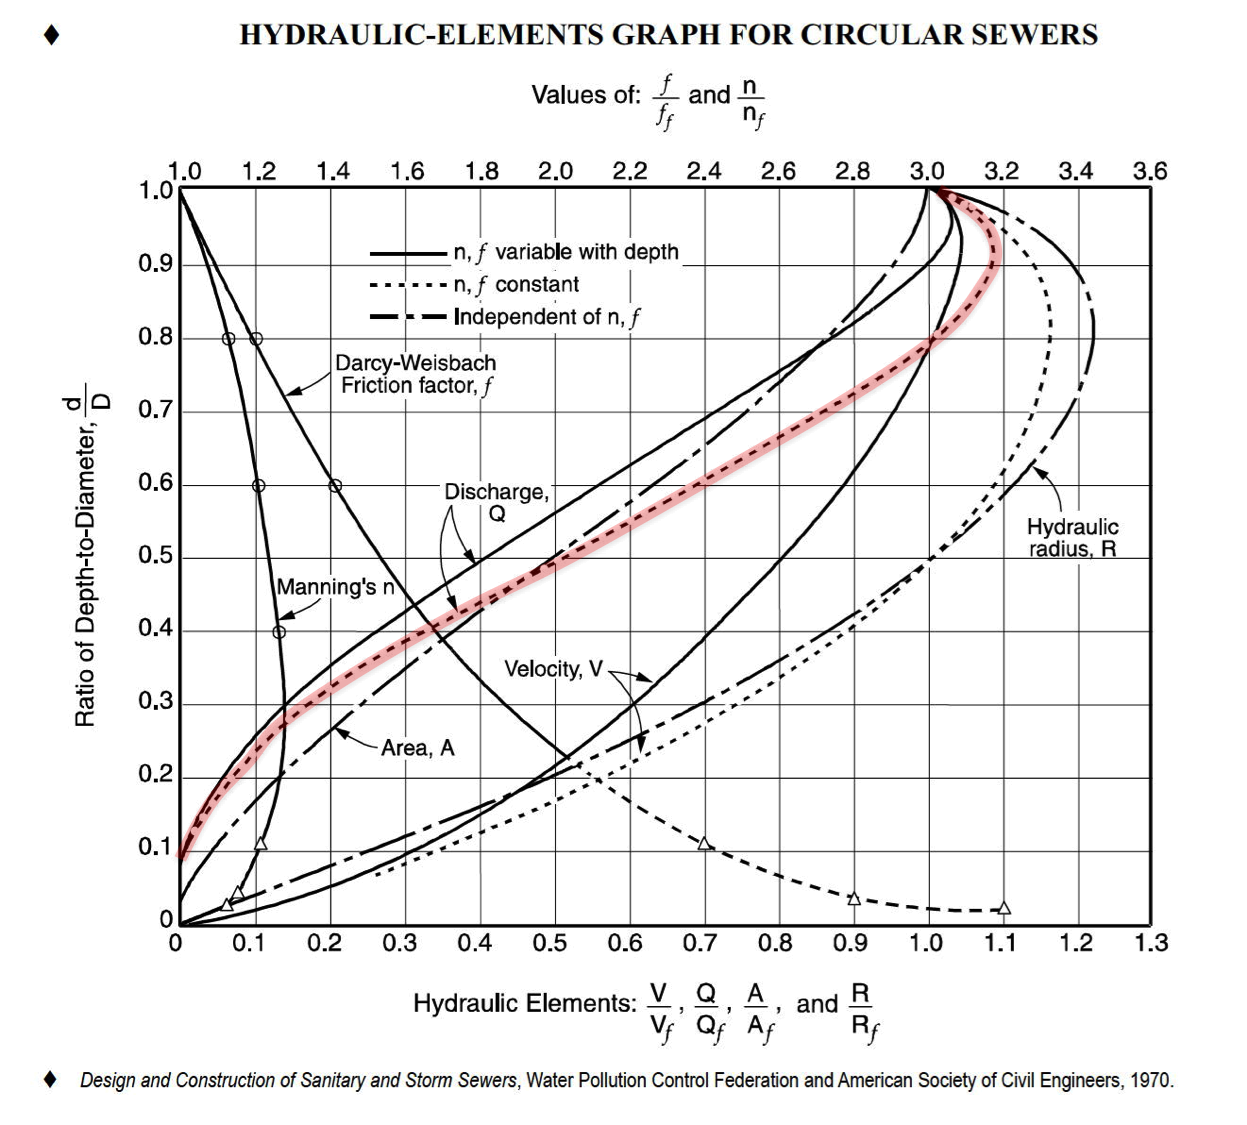
\includegraphics[width=4.5in]{hydraulic-elements.pdf}
   \caption{Hydraulic Elements Chart}
   \label{fig:hydraulic-elements} 
\end{figure}
\clearpage
\item What is the depth of actual flow in feet?
~\\
~\\
~\\
\item What is the depth of actual flow in inches?
~\\
~\\
~\\
\item Modify your sketch to include the water surface position and the approximate flow depth.
~\\
\item Is this portion of sewer close to surcharging?
~\\
\end{enumerate}

\clearpage
%%%%%%%%%%%%%%%%%%%%%%%%%%%%%%%%%%%%%%%%%%%%%%%%%
%%%%%%%%%%%PROBLEM 2 %%%%%%%%%%%%%%%%%%%%%%%%%%%%%%%
%%%%%%%%%%%%%%%%%%%%%%%%%%%%%%%%%%%%%%%%%%%%%%%%%
\item The questions on the following page refer to Figure \ref{fig:sewer} . 

\begin{figure}[ht!] %  figure placement: here, top, bottom, or page
\centering
   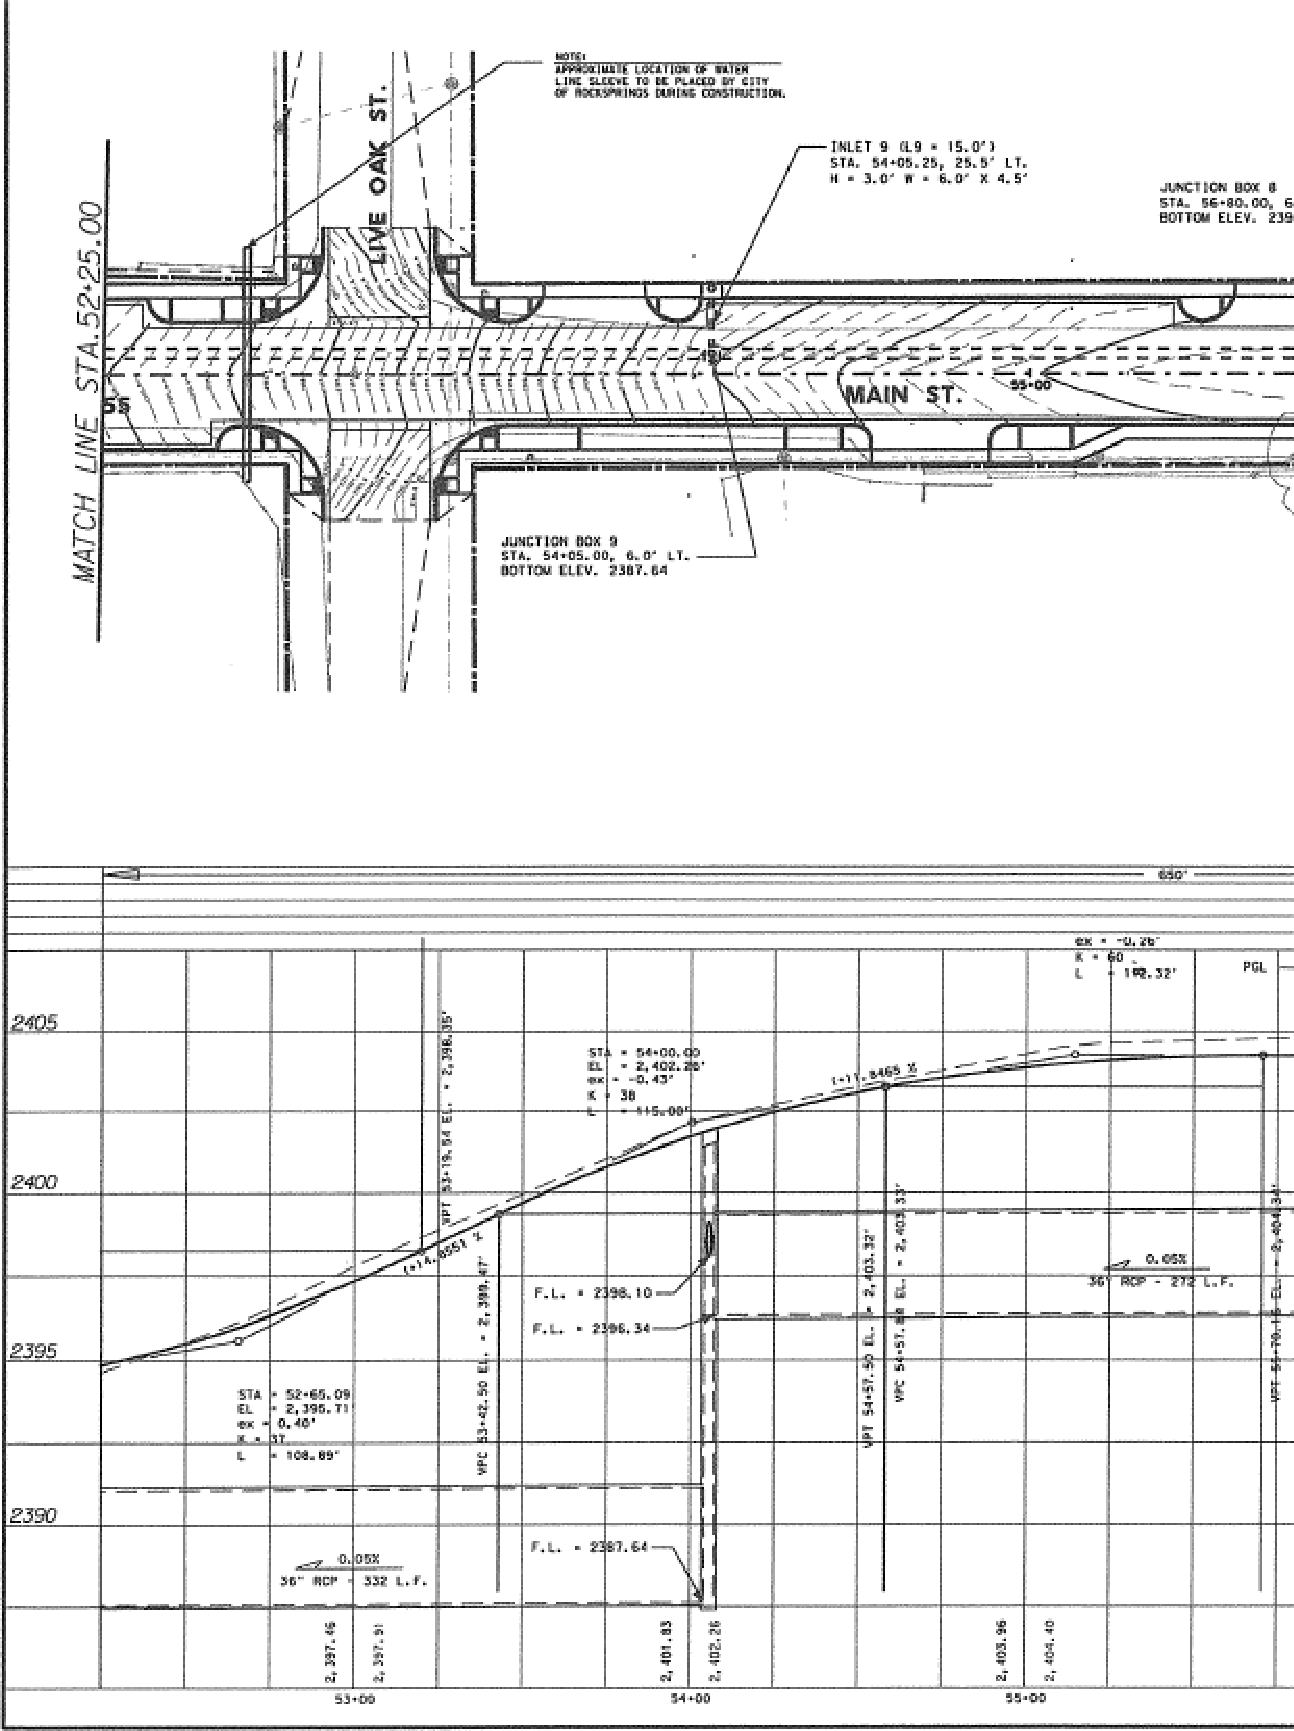
\includegraphics[width=5.5in]{sewer.pdf}
   \caption{Plan and profile of a storm sewer system}
   \label{fig:sewer} 
\end{figure}
\begin{enumerate}
\clearpage

\item Is the design flow in the drawing from left-to-right, or right-to-left?
~\\
~\\
\item The drawing indicates a drop at a junction box.  What is the bottom elevation of the junction box indicated on the drawing?
~\\
~\\
\item What is the diameter of the conduits indicated on the drawing?
~\\
~\\
\item What is the slope (in percent) of the storm sewer conduits?
~\\
~\\
\item Relative to the drop, what is the flow-line (invert) elevation of the left-most sewer pipe?
~\\
~\\
\item Relative to the drop, what is the flow-line (invert) elevation of the right-most sewer pipe?
~\\
~\\
\item Relative to the drop, what is the soffit (crown) elevation of the left-most sewer pipe?
~\\
~\\
\item Relative to the drop, what is the soffit (crown) elevation of the right-most sewer pipe?
~\\
~\\
\end{enumerate}
\clearpage
\item Figure \ref{fig:diameter-increase} is a plan-and profile of a portion of a storm sewer system.  Answer the questions on the following page.
\begin{figure}[ht!] %  figure placement: here, top, bottom, or page
\centering
   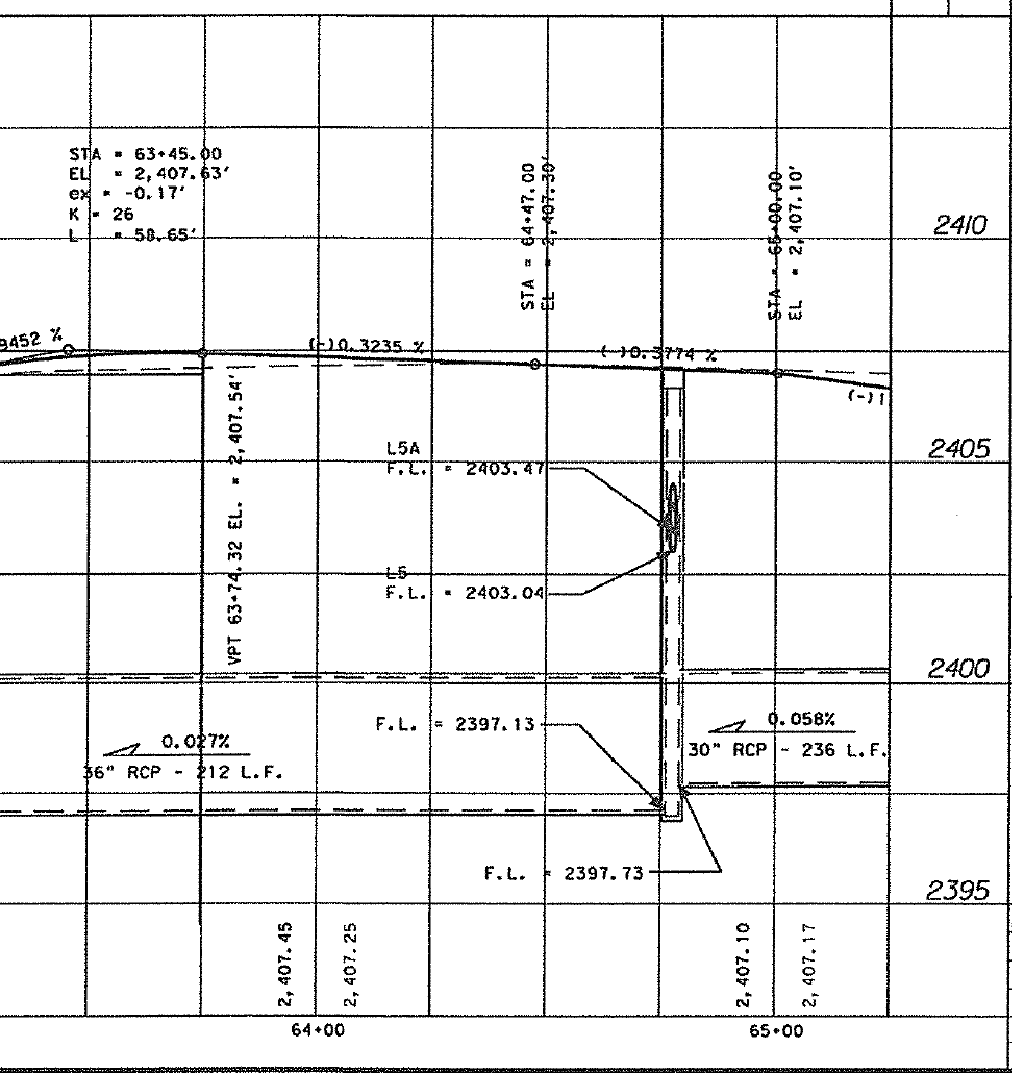
\includegraphics[width=5in]{diameter-increase.pdf}
   \caption{Plan and profile of a storm sewer system}
   \label{fig:diameter-increase} 
\end{figure}
\clearpage
\begin{enumerate}
\item What is the diameter of the conduit on the right-side of the drawing?
~\\
\item What is the slope of the conduit (in percent) on the right-side of the drawing?
~\\
\item What is the diameter of the conduit on the left-side of the drawing?
~\\
\item What is the slope of the conduit (in percent) on the right-side of the drawing?
~\\
\item What is the soffit (crown) elevation of the right-most sewer pipe?
~\\
\item What is the soffit (crown) elevation of the left-most sewer pipe?
~\\
\item What is the flow-line (invert) elevation of the right-most sewer pipe?
~\\
\item What is the flow-line (invert) elevation of the left-most sewer pipe?
~\\
\item Explain, using sketches as necessary, why sewer soffit elevations should match (or drop in the flow direction) at a junction when the pipe diameter increases moving downstream. 
\end{enumerate}

%%%%%%%%%%%%%%%%%%
% EPA-NET MSMD %%%%%%%%
%%%%%%%%%%%%%%%%%%
\item An EPA-NET simulation produced the  "full report" listed below.   
\begin{verbatim}
  **********************************************************************
  Link - Node Table:
  ----------------------------------------------------------------------
  Link           Start          End                Length  Diameter
  ID             Node           Node                   ft        in
  ----------------------------------------------------------------------
  1              2              3                    1000        12
  2              3              4                    1000        12
  3              2              5                    1000        12
  4              3              6                    1000        12
  5              5              6                    1000        12
  6              6              4                    1000        12
  7              1              2                    1000        12
  Node Results:
  ----------------------------------------------------------------------
  Node                Demand      Head  Pressure   Quality
  ID                     CFS        ft       psi          
  ----------------------------------------------------------------------
  2                     0.00     76.94     33.34      0.00
  3                     0.00     75.55     32.74      0.00
  4                     3.00     74.51     32.28      0.00
  5                     0.00     76.23     33.03      0.00
  6                     0.00     75.51     32.72      0.00
  1                    -3.00    100.00      0.00      0.00 Reservoir
  Link Results:
  ----------------------------------------------------------------------
  Link                  Flow  VelocityUnit Headloss    Status
  ID                     CFS       fps    ft/Kft
  ----------------------------------------------------------------------
  1                     1.76      2.25      1.39      Open
  2                     1.51      1.93      1.04      Open
  3                     1.24      1.57      0.71      Open
  4                     0.25      0.32      0.04      Open
  5                     1.24      1.57      0.71      Open
  6                     1.49      1.89      1.01      Open
  7                     3.00      3.82     23.06      Open
\end{verbatim}
\clearpage
Using the information contained in the EPA-NET report on the previous page:
\begin{enumerate}[a)]
\item How many pipes are in the network?
~\\
\item How many junctions (nodes) are in the network?
~\\
\item How many reservoirs/tanks are in the network?
~\\
\item Sketch the network, label the pipes, junctions, and reservoirs.   Indicate any demands at nodes.   Indicate the flow rates and flow directions on your sketch.
\end{enumerate}

\item  An EPA-NET simulation model for a reservoir-pump-network was constructed and operated for four (4) different operational scenarios.   Figure \ref{fig:epa-net-map} is a depiction of the network.   The numbers next to the nodes are Node\_ID values in the reports that follow, and the numbers next to the pipes are the Link\_ID values.  The network is supplied from a reservoir through a booster pump, both are depicted on Figure \ref{fig:epa-net-map}. 

\begin{figure}[h!] %  figure placement: here, top, bottom, or page
\centering
   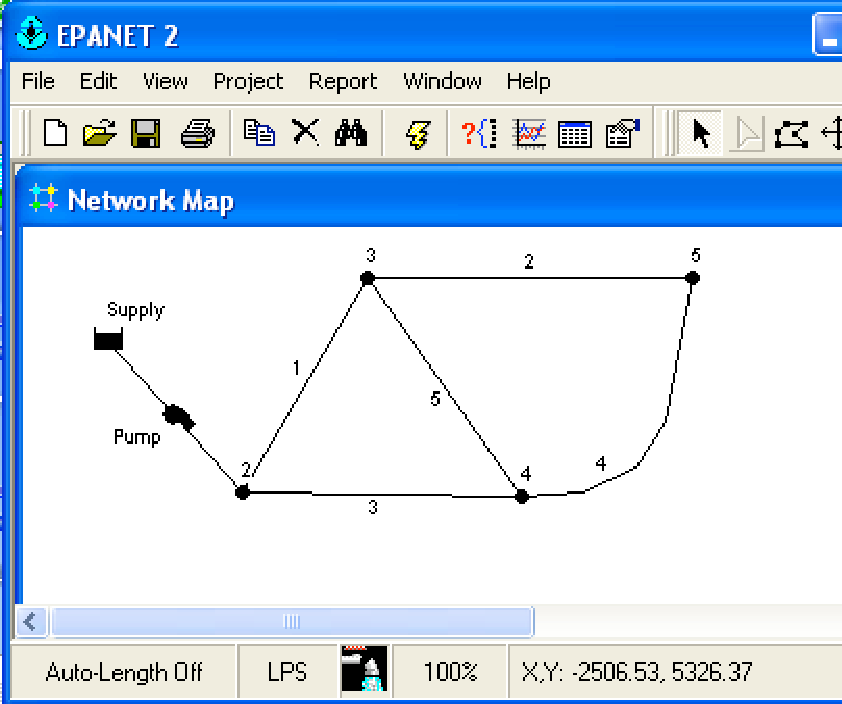
\includegraphics[width=3in]{epa-net-map.pdf}
   \caption{EPA-NET system topology.}
   \label{fig:epa-net-map} 
\end{figure}

Figure \ref{fig:epanet1} is the a portion of the summary report for simulation 1.   
Figure \ref{fig:epanet2} is the a portion of the summary report for simulation 2.  
Figure \ref{fig:epanet3} is the a portion of the summary report for simulation 3.  
Figure \ref{fig:epanet4} is the a portion of the summary report for simulation 4.

These four simulation represent different demand scenarios for the same system.



Interpret these reports, to answer the following questions:

\begin{enumerate}
\item Complete the table below.  $Q_{pump}$ is the discharge in liters-per-second through the pump station, $H_{Supply}$ is the head at the supply reservoir,  $H_{Node2}$ is the head at Node 2, and $\Delta H_{pump}$ is the added head supplied by the pump.
% Requires the booktabs if the memoir class is not being used
\begin{table}[htbp]
   \centering
      \caption{Pump Discharge and Supplied Head}
   \begin{tabular}{p{1in} p{1in} p{1in} p{1in} p{1in} } % Column formatting, @{} suppresses leading/trailing space
Simulation \# & $Q_{pump}$ & $H_{Supply}$ & $H_{Node2}$ & $\Delta H_{pump}$ \\
\hline
\hline
~~1 & ~ &~ & ~ & ~ \\
~ & ~ &~ & ~ & ~ \\
\hline
~~2 & ~ &~ & ~ & ~ \\
~ & ~ &~ & ~ & ~ \\
\hline
~~3 & ~ &~ & ~ & ~\\
~ & ~ &~ & ~ & ~ \\
\hline
~~4 & ~ &~ & ~ & ~ \\
~ & ~ &~ & ~ & ~ \\
\hline
   \end{tabular}
   \label{tab:pump-curve}
\end{table}

\item Complete the table below.  $Q_{pump}$ is the discharge in liters-per-second through the pump station, $\Delta H_{Node 2 -to- 5}$ is head loss in the system from Node 2 to Node 5.
\begin{table}[htbp]
   \centering
      \caption{System Discharge and Head Loss}
   \begin{tabular}{p{1in} p{1in} p{1in} p{1in} p{1in} } % Column formatting, @{} suppresses leading/trailing space
Simulation \# & $Q_{pump}$ & $H_{Node2}$ & $H_{Node5}$ & $\Delta H_{Node 2 -to- 5}$ \\
\hline
\hline
~~1 & ~ &~ & ~ & ~ \\
~ & ~ &~ & ~ & ~ \\
\hline
~~2 & ~ &~ & ~ & ~ \\
~ & ~ &~ & ~ & ~ \\
\hline
~~3 & ~ &~ & ~ & ~\\
~ & ~ &~ & ~ & ~ \\
\hline
~~4 & ~ &~ & ~ & ~ \\
~ & ~ &~ & ~ & ~ \\
\hline
   \end{tabular}
   \label{tab:system-curve}
\end{table}



\item If the pump performance curve has the mathematical structure: ~\\
$H_{pump} = H_{shutoff} - K_{pipe} \times Q^2$, estimate the values of $H_{shutoff}$  and $K_{pipe}$.
\\
\\
\\
\\
\\
\\
\\
\\
\\
\\
\\
\\
\\
\item If the system frictional loss curve has the mathematical structure:
 $H_{pipe}= K_{loss} \times Q^2$, estimate the value of $K_{loss}$

\clearpage
\item What effect would removing the pipe joining nodes 3 and 4 have on the system performance?   Explain your reasoning.
\\
\\
\\
\\
\\
\\
\\
\\
\\
\\
\\
\\
\\
\item Estimate the flow distribution and head losses the the system if the the pipe joining nodes 3 and 4 are removed, and the pipe joining node 4 and 5 is removed if the nodal demands are the same as SIMULATION  2.
\end{enumerate} 

%%% YOUR ON YOUR OWN %%%%%%%%%%%%%%%%%%%%
\begin{figure}[ht!] %  figure placement: here, top, bottom, or page
\centering

\begin{verbatim}
  Page 1                                            10/4/2010 2:27:47 PM
  **********************************************************************
  *                             E P A N E T                            *
  *                     Hydraulic and Water Quality                    *
  *                     Analysis for Pipe Networks                     *
  *                           Version 2.0                              *
  **********************************************************************
  Input File: SIMULATION #1
Link - Node Table:
  ----------------------------------------------------------------------
  Link           Start          End                Length  Diameter
  ID             Node           Node                    m        mm
  ----------------------------------------------------------------------
  1              2              3                    1000       124
  2              3              5                    1000       124
  3              2              4                    1000       124
  4              4              5                    1000       124
  5              3              4                    1400       124
  7              6              2                    #N/A      #N/A Pump
Node Results:
  ----------------------------------------------------------------------
  Node                Demand      Head  Pressure   Quality
  ID                     LPS         m         m          
  ----------------------------------------------------------------------
  2                     0.00     20.00     20.00      0.00
  3                     0.00     20.00     20.00      0.00
  4                     0.00     20.00     20.00      0.00
  5                     0.00     20.00     20.00      0.00
  6                     0.00      0.00      0.00      0.00 Reservoir
Link Results:
  ----------------------------------------------------------------------
  Link                  Flow  VelocityUnit Headloss    Status
  ID                     LPS       m/s      m/km
  ----------------------------------------------------------------------
  1                     0.00      0.00      0.00      Open
  2                     0.00      0.00      0.00      Open
  3                     0.00      0.00      0.00      Open
  4                     0.00      0.00      0.00      Open
  5                     0.00      0.00      0.00      Open
  7                     0.00      0.00    -20.00      Open Pump
  \end{verbatim}
     \caption{EPA-NET Summary Report, Simulation \#1}
   \label{fig:epanet1} 
\end{figure}


\begin{figure}[ht!] %  figure placement: here, top, bottom, or page
\centering
\begin{verbatim}
 Page 1                                            10/4/2010 2:28:15 PM
  **********************************************************************
  *                             E P A N E T                            *
  *                     Hydraulic and Water Quality                    *
  *                     Analysis for Pipe Networks                     *
  *                           Version 2.0                              *
  **********************************************************************
  Input File: SIMULATION 2
  Link - Node Table:
  ----------------------------------------------------------------------
  Link           Start          End                Length  Diameter
  ID             Node           Node                    m        mm
  ----------------------------------------------------------------------
  1              2              3                    1000       124
  2              3              5                    1000       124
  3              2              4                    1000       124
  4              4              5                    1000       124
  5              3              4                    1400       124
  7              6              2                    #N/A      #N/A Pump
  Node Results:
  ----------------------------------------------------------------------
  Node                Demand      Head  Pressure   Quality
  ID                     LPS         m         m          
  ----------------------------------------------------------------------
  2                     0.00     19.28     19.28      0.00
  3                     1.00     19.03     19.03      0.00
  4                     1.00     19.03     19.03      0.00
  5                     1.00     18.99     18.99      0.00
  6                    -3.00      0.00      0.00      0.00 Reservoir                                                              
  Link Results:
  ----------------------------------------------------------------------
  Link                  Flow  VelocityUnit Headloss    Status
  ID                     LPS       m/s      m/km
  ----------------------------------------------------------------------
  1                     1.50      0.12      0.25      Open
  2                     0.50      0.04      0.03      Open
  3                     1.50      0.12      0.25      Open
  4                     0.50      0.04      0.03      Open
  5                     0.00      0.00      0.00      Open
  7                     3.00      0.00    -19.28      Open Pump
  \end{verbatim}
     \caption{EPA-NET Summary Report, Simulation \#2}
   \label{fig:epanet2} 
\end{figure}

\begin{figure}[ht!] %  figure placement: here, top, bottom, or page
\centering

\begin{verbatim}
   Page 1                                            10/4/2010 2:29:00 PM
  **********************************************************************
  *                             E P A N E T                            *
  *                     Hydraulic and Water Quality                    *
  *                     Analysis for Pipe Networks                     *
  *                           Version 2.0                              *
  **********************************************************************
  Input File: SIMULATION 4
 Link - Node Table:
  ----------------------------------------------------------------------
  Link           Start          End                Length  Diameter
  ID             Node           Node                    m        mm
  ----------------------------------------------------------------------
  1              2              3                    1000       124
  2              3              5                    1000       124
  3              2              4                    1000       124
  4              4              5                    1000       124
  5              3              4                    1400       124
  7              6              2                    #N/A      #N/A Pump
Node Results:
  ----------------------------------------------------------------------
  Node                Demand      Head  Pressure   Quality
  ID                     LPS         m         m          
  ----------------------------------------------------------------------
  2                     0.00     17.12     17.12      0.00
  3                     2.00     16.16     16.16      0.00
  4                     2.00     16.16     16.16      0.00
  5                     2.00     16.04     16.04      0.00
  6                    -6.00      0.00      0.00      0.00 Reservoir
Link Results:
  ----------------------------------------------------------------------
  Link                  Flow  VelocityUnit Headloss    Status
  ID                     LPS       m/s      m/km
  ----------------------------------------------------------------------
  1                     3.00      0.25      0.96      Open
  2                     1.00      0.08      0.12      Open
  3                     3.00      0.25      0.96      Open
  4                     1.00      0.08      0.12      Open
  5                     0.00      0.00      0.00      Open
  7                     6.00      0.00    -17.12      Open Pump
  \end{verbatim}
     \caption{EPA-NET Summary Report, Simulation \#3}
   \label{fig:epanet3} 
\end{figure}

\begin{figure}[ht!] %  figure placement: here, top, bottom, or page
\centering

\begin{verbatim}
  Page 1                                            10/4/2010 2:29:46 PM
  **********************************************************************
  *                             E P A N E T                            *
  *                     Hydraulic and Water Quality                    *
  *                     Analysis for Pipe Networks                     *
  *                           Version 2.0                              *
  **********************************************************************
  Input File: SIMULATION 3
Link - Node Table:
  ----------------------------------------------------------------------
  Link           Start          End                Length  Diameter
  ID             Node           Node                    m        mm
  ----------------------------------------------------------------------
  1              2              3                    1000       124
  2              3              5                    1000       124
  3              2              4                    1000       124
  4              4              5                    1000       124
  5              3              4                    1400       124
  7              6              2                    #N/A      #N/A Pump
Node Results:
  ----------------------------------------------------------------------
  Node                Demand      Head  Pressure   Quality
  ID                     LPS         m         m          
  ----------------------------------------------------------------------
  2                     0.00     13.52     13.52      0.00
  3                     3.00     11.40     11.40      0.00
  4                     3.00     11.40     11.40      0.00
  5                     3.00     11.15     11.15      0.00
  6                    -9.00      0.00      0.00      0.00 Reservoir
 Link Results:
  ----------------------------------------------------------------------
  Link                  Flow  VelocityUnit Headloss    Status
  ID                     LPS       m/s      m/km
  ----------------------------------------------------------------------
  1                     4.50      0.37      2.12      Open
  2                     1.50      0.12      0.25      Open
  3                     4.50      0.37      2.12      Open
  4                     1.50      0.12      0.25      Open
  5                     0.00      0.00      0.00      Open
  7                     9.00      0.00    -13.52      Open Pump
  \end{verbatim}
     \caption{EPA-NET Summary Report, Simulation \#4}
   \label{fig:epanet4} 
\end{figure}
\clearpage
\clearpage
%%%%%%%%%%%%%%%%%%%%%%%%%%%%%%%%%%%%%%%%%%%

\begin{thebibliography}{}

\bibitem[\protect\citeauthoryear{Swamee and Jain}{Swamee and Jain}{1976}]{jain1976}
Swamee and Jain, A. K., 1976. Explicit equations for pipe-flow problems.  ASCE J. of Hyd. Div., 102(HY5) pp. 657-664 


\end{thebibliography}